\subsection*{Проект <<Станция метро>>}
\addcontentsline{toc}{subsection}{Проект <<Станция метро>>}

\textbf{Задание:}\\
Построить и проанализировать пешеходную имитационную модель станции метро Озерки.\\

\textbf{Решение:}\\
Имеется следующая схема станции метро Озерки. (Рисунок \ref{fig:metro_plan})
\begin{figure}[h]
	\centering 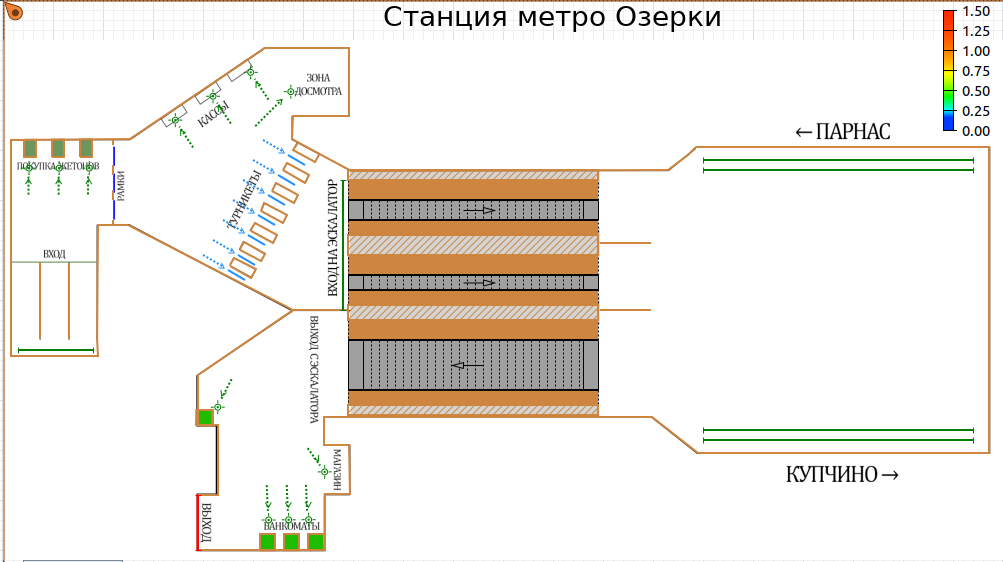
\includegraphics[scale=0.5]{metro_plan}
	\caption{Схема станции метро Озерки}
	\label{fig:metro_plan}
\end{figure}

При входе пассажиры могут купить жетоны либо в специальных автоматах, либо пойти на кассу, также их могут остановить на досмотр. После чего пассажиры проходят через турникеты и спускаются по эскалатору, далее они выбирают направление движения и садятся на поезд.\\

Соответственно, пассажиры, которые прибывают на станцию метро с других направлений, могут пройти по эскалатору на верх. После того как они поднялись, у них есть выбор пойти в группу банкоматов, пойти в <<непопулярный>> банкомат или зайти в магазин, также в магазине они смотрят на товар и в случае, если там нет нужного им продукта покинуть магазин или купить что-то. После всех данных альтернатив пассажиры покидают станцию метро.

\newpage

В соответствии с описанием данная модель была реализована в среде моделирования \textit{AnyLogic} (Рисунок \ref{fig:metro_anylogic_model}).

\begin{figure}[h]
	\centering 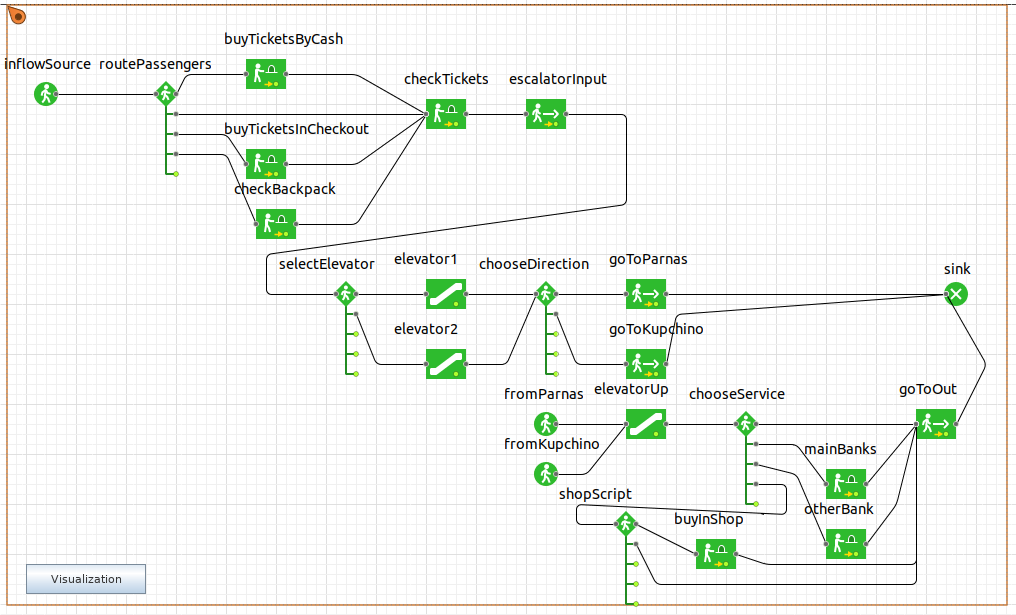
\includegraphics[scale=0.3]{metro_anylogic_model}
	\caption{Модель в среде \textit{AnyLogic}}
	\label{fig:metro_anylogic_model}
\end{figure}

Данная модель не имеет модификаций с изменением направления эскалатора и имеет статический потом интенсивности пассажиров.\\

Также в соседнем окне была построена визуализация модели и тепловая карта, которая соответствует плотности различных участков станции. (Рисунок \ref{fig:metro_visualization})

\begin{figure}[h]
	\centering 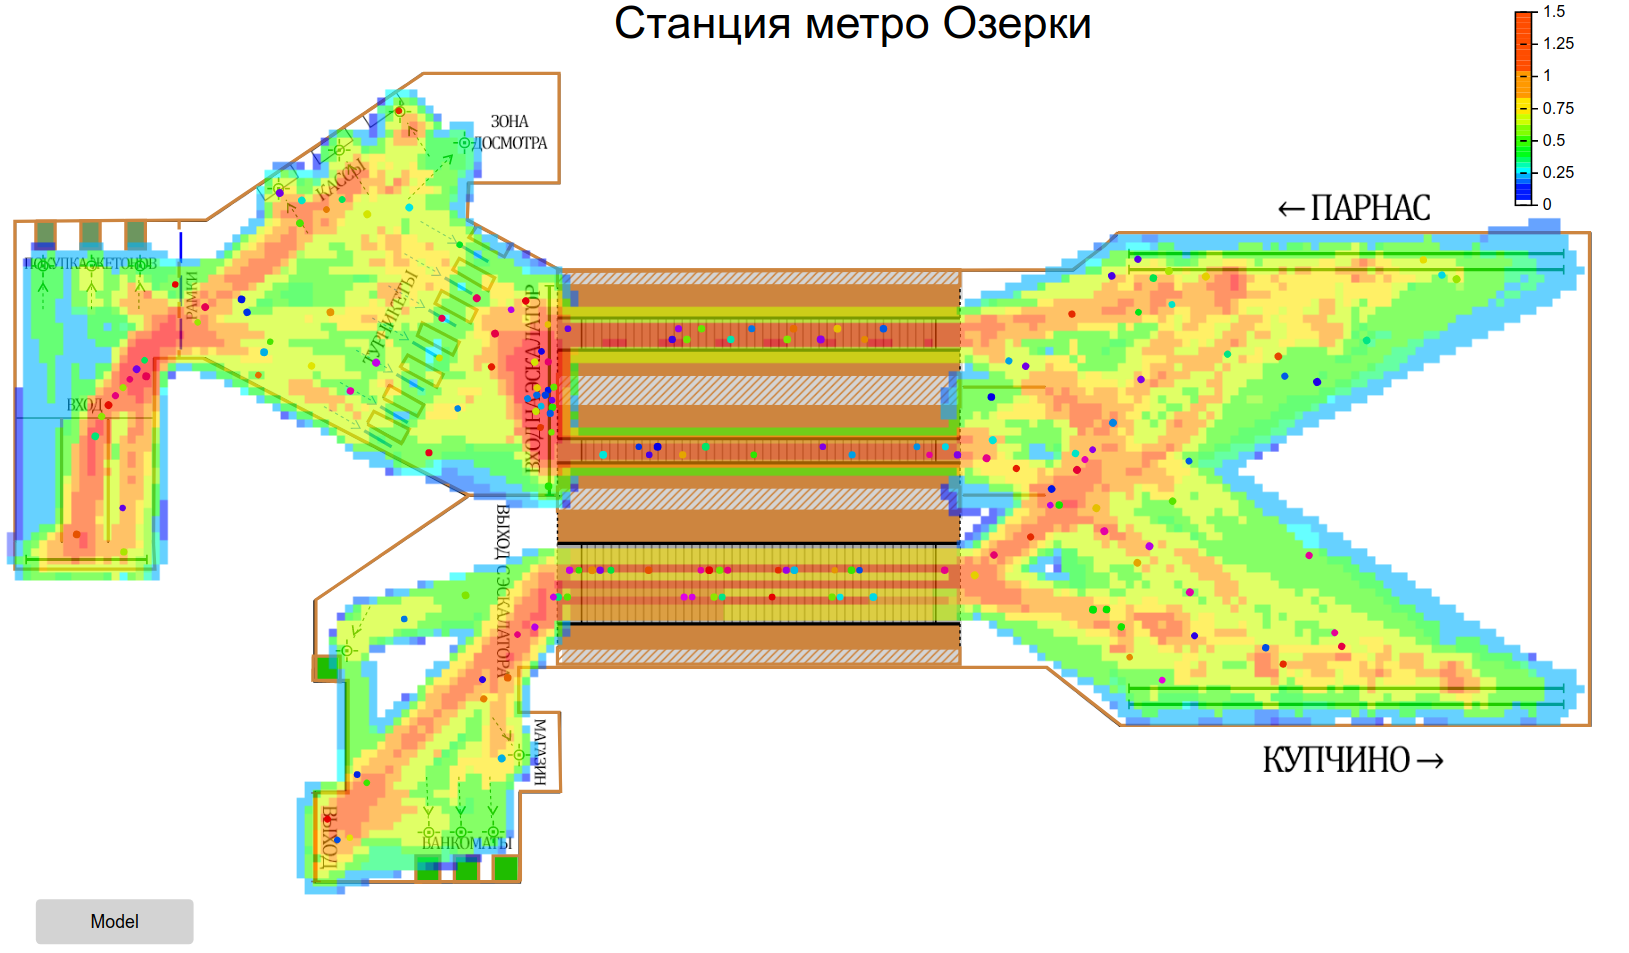
\includegraphics[scale=0.24]{metro_visualization}
	\caption{Модель в среде \textit{AnyLogic}}
	\label{fig:metro_visualization}
\end{figure}

\newpage

На данной тепловой карте можно видеть, что если средняя интенсивность пассажиропотока составляет 2000 человек в час, то <<узким горлышком>> на станции служит вход до рамок металлодетектора и входа на спуск по эскалатору.\\

Таким образом, нами была построена модель станции метро Озерки и была проанализирована зависимость плотности от различных факторов.